\chapter{Introduction}

\section{Mathematical Logic}
\subsection{Propositions}
Propositions are statements that can be either \true\ or \false.
\begin{example}
  \begin{itemize}
  \item The moon is smaller than the Earth (\true)
  \item $1+3=4$ (\true)
  \item Protons have no electric charge (\false)
  \item $12 > 13$ (\false)
  \end{itemize}
\end{example}

Propositions can be grouped together with \emph{operators}\index{Operator} such as \textbf{and}, \textbf{or}. The \textbf{and} operator returns a \true\ statement only if \textbf{both} the statements it groups are themselves \true, otherwise it returns \false.
\begin{example}
  Combining statements using the \textbf{and} operator (statememnts highlighted in \colorbox{col2!50}{blue} are true, statements highlighted in \colorbox{col1!50}{red} are false):
  \begin{align*}
  \thl{1+2=3} \text{ and } \thl{3-5=-2} &\Rightarrow \mtrue\\
  \thl{1+2=3} \text{ and } \fhl{2\times4=7} &\Rightarrow \false\\
  \fhl{\frac{10}{2}=1} \text{ and } \thl{2^{4}=16} &\Rightarrow \false\\
  \fhl{7<5} \text{ and } \fhl{10+2=13} &\Rightarrow \false\\
  \end{align*}
\end{example}

The \textbf{or} operator returns \true\ if \textbf{at least} one of the statements it groups is true.
\begin{example}
  Combining statements using the \textbf{or} operator (statememnts highlighted in \colorbox{col2!50}{blue} are true, statements highlighted in \colorbox{col1!50}{red} are false):
  \begin{align*}
  \thl{1+2=3} \text{ or } \fhl{3>7} &\Rightarrow \true\\
  \fhl{0+3=-1} \text{ or } \thl{1=1} &\Rightarrow \true\\
  \thl{2\times2=4} \text{ or } \thl{2+0=2} &\Rightarrow \true\\
  \fhl{3\times7=10} \text{ or } \fhl{\frac{1}{2}<\frac{1}{10}} &\Rightarrow \false\\
  \end{align*}
\end{example}

We can summarize this in a \emph{truth table}\index{Truth table}, for combinations of statements $A$ and $B$, which could each be either \true\ or \false:\\
~\\

\centering
\begingroup\setlength{\fboxsep}{0pt}
\colorbox{col2!10}{%
  \begin{tabular}[h]{p{1.5cm}p{1.5cm}p{1.5cm}p{1.5cm}}
  \rowcolor{col2!75}\multicolumn{4}{l}{\color{white}\textbf{Truth Table for the Operators AND, OR}}\\
  \rule{0pt}{4ex}
  $A$ & $B$ & AND & OR\\
  \midrule
  \true & \true & \true & \true \\
  \true & \false & \false & \true \\
  \false & \true & \false & \true \\
  \false & \false & \false & \false \\
  \midrule
  \end{tabular}
}\flushleft

The operators \textbf{and}, \textbf{or} and other operators have mathematical abbreviations (which are called \emph{notation}\index{Basic math notation}):
~\\~\\

\centering
\begingroup\setlength{\fboxsep}{0pt}
\colorbox{col2!10}{%
  \begin{tabular}{lll}
  \rowcolor{col2!75}\multicolumn{3}{l}{\color{white}\textbf{Common Mathematical Operators}}\\
  \rule{0pt}{4ex}
  Symbol & In words & Comments\\
  \midrule
  $\neg a$ & \textbf{not} $a$ & "Flips" \true\ to \false, and \false\ to \true.\\
  $a \wedge b$ & $a$ \textbf{and} $b$ & \\
  $a \vee b$ & $a$ \textbf{or} $b$ &\\
  $a \Rightarrow b$ & $a$ \textbf{implies} $b$ & "if $a$ is \true, then $b$ is also \true"\\
  $a \Leftrightarrow b$ & $a$ \textbf{is equivalent to} $b$ & "if and only if $a$ is \true, then $b$ is \true".\\
  $\forall x$ & \textbf{For all} $x$ (...) & \\
  $\exists x$ & \textbf{There exists} $x$ \textbf{such that} (...) & \\
  $a\defeq b$ & $a$ \textbf{is defined to be} $b$ & \\
  \midrule
  \end{tabular}
}\flushleft

\section{Sets}
\subsection{Basic Properties}
A \emph{set}\index{Set} is a collection of \emph{elements}\index{Elements (of a set)}. Elements of a set can be any concept - be it physical (a chair, a car, a tapir) or abstract (a number, an idea). In fact, elements of a set can themselves be sets. In this course we limit ourselves to only sets of numbers and other mathematical objects. Sets can have a \emph{finite} number of elements (for example, the set of all people) - or an \emph{infinite} number of elements (for example, the set of all numbers bigger than $3$).

We use curly brackets for notating sets.
\begin{example}
  \begin{equation*}
  \left\{ 1, 2, 3, 4 \right\}, \left\{ -3, 7, \pi, 0.1, 1337, \frac{1}{17} \right\}
  \end{equation*}
\end{example}

The order of elements in a set does not matter.
\begin{example}
  The follows sets are all equal:
  \begin{equation*}
  \left\{ 1,2,3,4 \right\} = \left\{ 1,3,2,4 \right\} = \left\{ 4,1,2,3 \right\}
  \end{equation*}
\end{example}

There are no repetitions in a set.
\begin{example}
  \begin{equation*}
  \left\{ 1,2,3,3,3,4 \right\} = \left\{ 1,2,3,4 \right\}.
  \end{equation*}
\end{example}

Sets are usually designated by upper-case letters, while their elements are usually designated with lower-case letters.
\begin{example}
  \begin{equation*}
  A=\left\{ 0,3,-1 \right\}, B=\left\{ -7, \pi, 0, \frac{1}{2} \right\}
  \end{equation*}
\end{example}

The symbol $\in$ means that an element is in a set, and $\notin$ means that an element is not in a set.
\begin{example}
  For the sets $A,B$ defined above:
  \begin{equation*}
  3\in A,\ 4\notin A,\ \pi\in B,\ 1\notin B
  \end{equation*}
\end{example}

We can also define sets using a proposition.
\begin{example}
  \begin{equation*}
  M = \left\{ x \mid x>1 \text{ and } x<3  \right\}
  \end{equation*}
\end{example}
The vertical line separator $\mid$ means "such that", and so the set $M$ is defined as "$x$ such that $x$ is bigger than $1$ and smaller than $3$". An alternative notation would be
\begin{equation*}
  M = \left\{ x \mid 1<x<3 \right\}
\end{equation*}

\begin{warning}
For the above set, $1\notin M$ and also $3\notin M$. This is because of the use of $<$ (\emph{smaller than}), and not $\leq$ (\emph{smaller than or equal to}).
\end{warning}

The number of elements in a set (also called its \emph{cardinality}\index{Cardinality}) is notated with two vertical bars.
\begin{example}
  \begin{equation*}
  M=\left\{ 1,4,6,13,17 \right\} \Rightarrow \left| M \right|=5
  \end{equation*}
\end{example}

A special set is the \emph{empty set}\index{Empty set}, notated as $\emptyset$. It has the unique property that $\left| \emptyset \right|=0$.

\subsection{Subsets and Supersets}
If $A$ contains all elements of $B$ (and perhaps other elements as well), then $A$ is a \emph{superset}\index{Superset} of $B$, and $B$ is a \emph{subset}\index{Subset} of $A$.
\begin{example}
  The sets $\left\{ 0,-3 \right\}, \left\{ 2,-5,7 \right\}, \left\{ 1,-3,0 \right\}$ are all subsets of $\left\{ 1,2,-5,-3,0,7 \right\}$.
  (these are not \textbf{all} the subsets of $\left\{ 1,2,-5,-3,0,7 \right\}$, only three examples)
\end{example}

The superset/subset relation between $A$ and $B$ is written as
\begin{equation*}
  B\subseteq A
\end{equation*}
Using a \emph{Venn diagram}\index{Venn diagram}, we could visualize this as follows:
\begin{figure}[H]
  \centering
  \begin{tikzpicture}
  \def\firstcircle{(0,0) circle (2)}
  \def\secondcircle{(0.5,1) circle (0.75)}
  \begin{scope}
  \fill[col1!50]\firstcircle;
  \fill[col2!50]\secondcircle;
  \draw \firstcircle node[below] {$A$};
  \draw \secondcircle node [above] {$B$};
  \end{scope}
  \end{tikzpicture}
\end{figure}

If for some two sets $M,N$ both $M\subseteq N$ and $N\subseteq M$, then both sets are identical. Writing this formally:
\begin{equation*}
  M\subseteq N \wedge N\subseteq M \Leftrightarrow N=M
\end{equation*}

\subsection{Intersections and Unions}
We define the \emph{intersection}\index{Intersection} of two sets $A,B$ as the set of all elements that are \emph{both} in $A$ \textbf{and} in $B$.

\begin{example}
  Given the sets $A=\left\{ 1,2,5,6,7 \right\}$ and $B=\left\{ -1,0,1,5,10,13,15 \right\}$, the intersection of $A$ and $B$ is $\left\{ 1, 5 \right\}$.
\end{example}

The symbol denoting intersection is $\cap$. An intersection can be formally defined as
\begin{equation*}
  A\cap B = \left\{ x \mid x\in A \wedge x\in B \right\}
\end{equation*}
(read: "the intersection of $A$ and $B$ is the set containing all elements $x$, such that $x$ is in $A$ and $x$ is in $B$")

A Venn diagram visualization of $A\cap B$ (green area):
\begin{figure}[H]
  \centering
  \begin{tikzpicture}
  \def\firstcircle{(0,0) circle (2)}
  \def\secondcircle{(2.3,0) circle (1.5)}
  \fill[col1!50]\firstcircle;
  \fill[col2!50]\secondcircle;
  \begin{scope}
  \clip \firstcircle;
  \fill[col3!50]\secondcircle;
  \end{scope}
  \draw\firstcircle node[below] {$A$};
  \draw\secondcircle node[above] {$B$};
  \draw (1.4,-0.2) node[above] {$A\cap B$};
  \end{tikzpicture}
\end{figure}

If the intersection of two sets is empty ($A\cap B=\emptyset$), then the sets are said to be \emph{disjoint}\index{Disjoint sets}:
\begin{figure}[H]
  \centering
  \begin{tikzpicture}
  \def\firstcircle{(0,0) circle (2)}
  \def\secondcircle{(4,0) circle (1.5)}
  \fill[col1!50]\firstcircle;
  \fill[col2!50]\secondcircle;
  \draw\firstcircle node[below] {$A$};
  \draw\secondcircle node[above] {$B$};
  \end{tikzpicture}
\end{figure}

The \emph{union}\index{Union of sets} of two sets $A,B$ is the set of all elements that are either in $A$ or in $B$ (or both).
\begin{example}
  The union of the sets $A=\left\{	-5, 7, 1\right\}$ and $B=\left\{ 10, -2, -5, 2 \right\}$ is $$A\cup B=\left\{ 10, -2, -5, 2, 7, 1 \right\}.$$
\end{example}

The symbol denoting union is $\cup$. A union can be formally defined as
\begin{equation*}
  A\cup B = \left\{ x \mid x\in A \vee x\in B \right\}
\end{equation*}
(read: "the union of $A$ and $B$ is the set containing all elements $x$, such that $x$ is in $A$ or $x$ is in $B$")

A Venn diagram visualization of $A\cup B$ (purple area):
\begin{figure}[H]
  \centering
  \begin{tikzpicture}
  \def\firstcircle{(0,0) circle (2)}
  \def\secondcircle{(2.3,0) circle (1.5)}
  \fill[col4!50, draw=black]\firstcircle;
  \fill[col4!50, draw=black]\secondcircle;
  \draw\firstcircle node {$A$};
  \draw\secondcircle node {$B$};
  \end{tikzpicture}
\end{figure}

What is the number of elements in $A\cup B$? Let's look at an example: $A=\left\{ 1,2,3,4,5 \right\},\ B=\left\{ 4,5,6,7 \right\}$. We can see that $|A|=5,\ |B|=4$. The union of $A,B$ is $A\cup B = \left\{ 1,2,3,4,5,6,7 \right\}$, and $\left|A\cup B\right|=7$. If we just count each element in both sets, we will have $9$ elements: $1,2,3,6$ and $7$ are each counted once, but $4$ and $5$ are each counted twice (because they are both in $A$ and in $B$). To account for this double count, we can simply subtract $2$ - the number of elements that are in both sets. This is exactly $\left|A\cap B\right|$ (the number of elements in the intersection of $A$ and $B$). Hence, for two sets $A,B$, this always holds:
\begin{equation*}
  \left|A\cup B\right| = |A| + |B| - \left|A\cap B\right|
\end{equation*}
Note that if $A,B$ are disjoint, $\left|A\cup B\right| = |A| + |B|$ (because $\left|A\cap B\right|=0$).

\subsection{Difference of Sets}
The \emph{difference}\index{Difference of a set} of $A$ and $B$ is the set of all elements in $A$ that \emph{are not} elements of $B$. This is written as $A-B$ (or sometimes $A\setminus B$). Example:
\begin{equation*}
  A = \left\{ 1,5,9,10 \right\},\ B=\left\{ -3,2,5,9,13 \right\},\ A-B=\left\{ 1,10 \right\}
\end{equation*}
Formally:
\begin{equation*}
  A-B = \left\{ x \mid x\in A,\ x\notin B\right\}
\end{equation*}

A Venn diagram visualization of $A-B$ (orange area):
\begin{figure}[H]
  \centering
  \begin{tikzpicture}
  \def\firstcircle{(0,0) circle (2)}
  \def\secondcircle{(2.3,0) circle (1.5)}
  \begin{scope}
  \begin{scope}[even odd rule]% first circle without the second
  \clip \secondcircle (-3,-3) rectangle (3,3);
  \fill[col5!50] \firstcircle;
  \end{scope}
  \draw \firstcircle node {$A$};
  \draw \secondcircle node {$B$};
  \end{scope}
  \end{tikzpicture}
\end{figure}

\subsection{Complement}
The \emph{complement}\index{Complement of a set} of a set $A$ in a reltaion to a superset $Z\supset A$ is the difference $Z-A$, and is notated $A^{\mathsf{c}}$.
\begin{example}
  $Z=\left\{ 1,2,3,4,5 \right\}, A=\left\{ 1,2,3 \right\} \Rightarrow A^{\mathsf{c}}=\left\{ 4,5 \right\}$.
\end{example}
Formally:
\begin{equation*}
  A^{\mathsf{c}} = \left\{ x\in Z \mid x\notin A \right\}
\end{equation*}
A Venn diagram representation:
\begin{figure}[H]
  \centering
  \begin{tikzpicture}
  \def\firstcircle{(0,0) circle (3)}
  \def\secondcircle{(1.3,1) circle (1)}
  \fill[col1!50, draw=black]\firstcircle;
  \fill[col2!50, draw=black]\secondcircle;
  \node at (1.3,1) {$A$};
  \node at (0,0) {$A^{\mathsf{c}}$};
  \node at (-2.7,1.9) {$Z$};
  \end{tikzpicture}
\end{figure}
\subsection{Power Set}
The set of all subsets of a given set $A$ is called the \emph{powerset of $A$}\index{Powerset}.
\begin{example}
  $A=\left\{ 1,2,3 \right\}$. All the subsets of $A$ are:
  \begin{equation*}
  \emptyset, \left\{ 1 \right\}, \left\{ 2 \right\}, \left\{ 3 \right\}, \left\{ 1,2 \right\}, \left\{ 1,3 \right\}, \left\{ 2,3 \right\}, \left\{ 1,2,3 \right\}.
  \end{equation*}
  Thus, the power set of $A$ is
  \begin{equation*}
  P(A) = \left\{ \emptyset, \left\{ 1 \right\}, \left\{ 2 \right\}, \left\{ 3 \right\}, \left\{ 1,2 \right\}, \left\{ 1,3 \right\}, \left\{ 2,3 \right\}, \left\{ 1,2,3 \right\} \right\}.
  \end{equation*}
\end{example}
\begin{warning}
  The empty set $\emptyset$ is a subset of all sets. Each set is also a subset of itself.
\end{warning}

\subsection{Important Number Sets}
Some important sets of numbers, that will be used frequently in the course (all of them have infinite number of elements):
\begin{itemize}
  \item \textbf{The natural numbers} (symbol: $\mathbb{N}$). These are the numbers $1,2,3,\dots$.
  \item \textbf{The integers} (symbol: $\mathbb{Z}$). These are the "whole numbers" (i.e. not fractions). They include all the natural numbers together with their negatives (i.e. $-1,-2,-3,\dots$) and $0$.
  \item \textbf{The rational} numbers (symbol: $\mathbb{Q}$). As their name suggests, they are ratios between two integers (e.g. $\frac{1}{2},\ \frac{-5}{3},\ \frac{7}{13}$).
  \item \textbf{The real numbers} (symbol: $\mathbb{R}$). These are all the numbers on the number line (e.g. $2, \pi, \frac{\sqrt{3}}{17}, \sqrt{5}, -7.2, e^{\pi}$). A proper definition of the real numbers is beyond the scope of this course.
  \item \textbf{The complex numbers} (symbol: $\mathbb{C}$). These are numbers of the form $a+bi$, where $a,b$ are real numbers, and $i=\sqrt{-1}$.
\end{itemize}
~\\~\\

\centering
\begingroup\setlength{\fboxsep}{0pt}
\colorbox{col2!10}{%
\begin{tabular}{lll}
  \rowcolor{col2!75}\multicolumn{3}{l}{\color{white}\textbf{Important Number Sets}}\\
  \rule{0pt}{4ex}
  Symbol & Name & Definition \\
  \midrule
  $\mathbb{N}$ & Natural numbers & $\left\{1,2,3,4,\dots\right\}$\\
  $\mathbb{Z}$ & Integers & $\left\{ 0,\pm x \mid x\in\mathbb{N} \right\}$\\
  $\mathbb{Q}$ & Rational numbers & $\left\{ \frac{p}{q} \mid p\in\mathbb{Z}, q\in\mathbb{N} \right\}$\\
  $\mathbb{R}$ & Real numbers & \\
  $\mathbb{C}$ & Complex numbers & $\left\{ a+ib \mid a,b\in\mathbb{R}, i=\sqrt{-1} \right\}$\\
  \midrule
\end{tabular}
}\flushleft

The relations between these sets are
\begin{equation*}
  \mathbb{N}\subset \mathbb{Z}\subset\mathbb{Q}\subset\mathbb{R}\subset\mathbb{C}
\end{equation*}
(the symbol $\subset$ means "a proper subset")

\begin{warning}
  Although each of these sets is infinite, the actual number of elements in $\mathbb{R}$ and $\mathbb{C}$ is bigger than the number of elements in $\mathbb{N},\mathbb{Z}$ and $\mathbb{Q}$. There are different kinds of infinities.
\end{warning}

\subsection{Cartesian Products}
The \emph{cartesian product}\index{Cartesian product} of two sets $A,B$, denoted $A\times B$, is the set of all possible \textbf{ordered} pairs, where the first component is an element of $A$ and the second component is an element of $B$.
\begin{example}
  Consider $A=\left\{ 1,2,3 \right\},\ B=\left\{ x, y \right\}$. Then:
  \begin{equation*}
  A\times B = \left\{ \left( 1,x \right), \left( 1,y \right), \left( 2,x \right), \left( 2,y \right), \left( 3,x \right), \left( 3,y \right) \right\}
  \end{equation*}
\end{example}

\begin{warning}
  Since the elements of a cartesian product are \textbf{ordered} pairs, $A\times B\neq B\times A$ (unless $A=B$).
\end{warning}

Formally:
\begin{equation*}
  A\times B = \left\{ \left( a,b \right) \mid a\in A,\	b\in B \right\}
\end{equation*}

The number of elements in a cartesian product is
\begin{equation*}
  \left|A\times B\right| = |A|\cdot|B|
\end{equation*}

The definition of a cartesian product can be expanded to $n\in\mathbb{N}$ sets $A_{1}, A_{2}, \dots, A_{n}$:
\begin{equation*}
  A_{1}\times A_{2} \times \dots \times A_{n} = \left\{ \left(a_{1}, a_{2}, \dots, a_{n}\right) \mid a_{1}\in A_{1}, a_{2}\in A_{2}, \dots, a_{n}\in A_{n} \right\}
\end{equation*}
or more compactly:
\begin{equation*}
  \prod\limits_{i=1}^{n} A_{i} = \left\{ \left( a_{1}, a_{2}, \dots, a_{i} \right) \mid a_{i}\in A_{i}, i=1,2,\dots,n\right\}
\end{equation*}
The symbol $\prod$ is a generalized product notation. It will be discussed in more details later in the course.

A cartesian product of the same set is written in an similar way to a power. For example
\begin{align*}
  \mathbb{R}\times\mathbb{R} &= \mathbb{R}^{2}\\
  \mathbb{R}\times\mathbb{R}\times\mathbb{R} &= \mathbb{R}^{3}
\end{align*}
These are, respectively, sets of pairs of real numbers, e.g. $\left( -3,1 \right), (\pi,2), (-\frac{\sqrt{7}}{13}, 0)$, and triples of real numbers, e.g. $\left( 1,2,-\pi \right), \left( -6,\frac{1}{\sqrt{\pi}}, 0.2 \right), \left( \frac{1}{51}, \sqrt{3}, -4 \right)$.

\begin{example}
  \begin{align*}
  A=\left\{ a,b \right\}\ &\Rightarrow\ A^{3}=\left\{\left( a,a,a \right), \left( a,a,b \right), \left( a,b,a \right), \left( a,b,b \right), \left( b,a,a \right), \left( b,a,b \right), \left( b,b,a \right), \left( b,b,b \right)\right\}.\\
  B=\left\{ 1,2,3 \right\}\ &\Rightarrow\ B^{2}=\left\{\left( 1,1 \right), \left( 1,2 \right), \left( 1,3\right), \left( 2,1 \right), \left( 2,2 \right), \left( 2,3 \right), \left( 3,1 \right),\left( 3,2 \right), \left( 3,3 \right)\right\}.
  \end{align*}
\end{example}

\section{Functions}
\subsection{Relations}
A \emph{relation}\index{Relation between two sets} between two sets $A,B$ is a way to "connect" the elements in the two sets in pairs. It is a subset of the cartesian product $A\times B$.
\begin{example}
  A relation $R$ between the sets $A=\left\{ 1,2,3,4,5 \right\}$ and $B=\left\{ \alpha,\beta,\gamma \right\}$. 
  \begin{figure}[H]
  \centering
  \begin{tikzpicture}
  \fill[col1!20, draw=col1, thick] (0,0) circle [x radius=0.75, y radius=2]; 
  \node (A1) at (0,1.5) {1};
  \node (A2) at (0,0.75) {2};
  \node (A3) at (0,0) {3};
  \node (A4) at (0,-0.75) {4};
  \node (A5) at (0,-1.5) {5};
  \node[above=5mm of A1] {\color{col1}$A$};

  \fill[col2!20, draw=col2, thick] (2,0) circle [x radius=0.75, y radius=1.5]; 
  \node (B1) at (2,1) {$\alpha$};
  \node (B2) at (2,0) {$\beta$};
  \node (B3) at (2,-1) {$\gamma$};
  \node[above=5mm of B1] {\color{col2}$B$};

  \draw[->, thick] (A1) -- (B1);
  \draw[->, thick] (A2) -- (B1);
  \draw[->, thick] (A3) -- (B2);
  \draw[->, thick] (A5) -- (B3);
  \end{tikzpicture}
  \end{figure}
  Notice how not all elements are connected (for example, $4$ is not connected to any element in $B$), and some elements in $A$ are connected to the same element in $B$ ($1,2$ are both connected to $\alpha$). The pairs making up the relation $R$ are $\left( 1,\alpha \right), \left( 2,\alpha \right), \left( 3,\beta \right), \left( 5,\gamma \right)$, which are all elements of the cartesian product $A\times B$.
\end{example}

Reversing the connections yields $R^{-1}$, which is a subset of $B\times A$.
\begin{example}
  The converse relation $R^{-1}$ for the above relation $R$ between $A$ and $B$.
  \begin{figure}[H]
  \centering
  \begin{tikzpicture}
  \fill[col1!20, draw=col1, thick] (0,0) circle [x radius=0.75, y radius=2]; 
  \node (A1) at (0,1.5) {1};
  \node (A2) at (0,0.75) {2};
  \node (A3) at (0,0) {3};
  \node (A4) at (0,-0.75) {4};
  \node (A5) at (0,-1.5) {5};
  \node[above=5mm of A1] {\color{col1}$A$};
  
  \fill[col2!20, draw=col2, thick] (2,0) circle [x radius=0.75, y radius=1.5]; 
  \node (B1) at (2,1) {$\alpha$};
  \node (B2) at (2,0) {$\beta$};
  \node (B3) at (2,-1) {$\gamma$};
  \node[above=5mm of B1] {\color{col2}$B$};

  \draw[<-, thick] (A1) -- (B1);
  \draw[<-, thick] (A2) -- (B1);
  \draw[<-, thick] (A3) -- (B2);
  \draw[<-, thick] (A5) -- (B3);
  \end{tikzpicture}
  \end{figure}
  The pairs making up the relation $R^{-1}$ are $\left( \alpha,1 \right), \left( \alpha,2 \right), \left( \beta,3 \right), \left( \gamma,5 \right)$, which are all elements of the cartesian product $B\times A$. 
\end{example}

\subsection{Basic Definition of a Function}
A \emph{function}\index{Function} between the sets $A,B$ is a relation in which for every element $a\in A$ there is exactly \textbf{one} connection to an element $b\in B$.
\begin{warning}
  A function can have more than one element $a\in A$ connected to the same element $b\in B$. The only restriction is that no element $a\in A$ is connected to \textbf{more than one} element $b\in B$.
\end{warning}
\begin{example}
  A valid function from $A$ to $B$:
  \begin{figure}[H]
  \centering
  \begin{tikzpicture}
  \fill[col1!20, draw=col1, thick] (0,0) circle [x radius=0.75, y radius=2]; 
  \node (A1) at (0,1.5) {1};
  \node (A2) at (0,0.75) {2};
  \node (A3) at (0,0) {3};
  \node (A4) at (0,-0.75) {4};
  \node (A5) at (0,-1.5) {5};
  \node[above=5mm of A1] {\color{col1}$A$};
  
  \fill[col2!20, draw=col2, thick] (2,0) circle [x radius=0.75, y radius=1.75]; 
  \node (B1) at (2,1.2) {$\alpha$};
  \node (B2) at (2,0.4) {$\beta$};
  \node (B3) at (2,-0.4) {$\gamma$};
  \node (B4) at (2,-1.2) {$\delta$};
  \node[above=5mm of B1] {\color{col2}$B$};

  \draw[->, thick] (A1) -- (B1);
  \draw[->, thick] (A2) -- (B1);
  \draw[->, thick] (A3) -- (B2);
  \draw[->, thick] (A4) -- (B4);
  \draw[->, thick] (A5) -- (B3);
  \end{tikzpicture}
  \end{figure}
  An invalid function from $A$ to $B$ (connections in red cause invalidity):
  \begin{figure}[H]
  \centering
  \begin{tikzpicture}
  \fill[col1!20, draw=col1, thick] (0,0) circle [x radius=0.75, y radius=2]; 
  \node (A1) at (0,1.5) {1};
  \node (A2) at (0,0.75) {2};
  \node (A3) at (0,0) {3};
  \node (A4) at (0,-0.75) {4};
  \node (A5) at (0,-1.5) {5};
  \node[above=5mm of A1] {\color{col1}$A$};
  
  \fill[col2!20, draw=col2, thick] (2,0) circle [x radius=0.75, y radius=1.75]; 
  \node (B1) at (2,1.2) {$\alpha$};
  \node (B2) at (2,0.4) {$\beta$};
  \node (B3) at (2,-0.4) {$\gamma$};
  \node (B4) at (2,-1.2) {$\delta$};
  \node[above=5mm of B1] {\color{col2}$B$};

  \draw[->, thick] (A1) -- (B1);
  \draw[->, thick] (A2) -- (B1);
  \draw[->, thick] (A3) -- (B2);
  \draw[->, thick] (A4) -- (B4);
  \draw[->, thick, red] (A5) -- (B3);
  \draw[->, thick, red] (A5) -- (B2);
  \end{tikzpicture}
  \end{figure}
\end{example}

\subsection{Domain and Image of a Function}
We notate that a function $f$ connects each element $a\in A$ to an element $b\in B$ by writing 
\begin{equation*}
  f:A\to B.
\end{equation*}
The set $A$ is then the \emph{domain}\index{Domain of a function} of $f$, while $B$ is the \emph{image}\index{Image of a function} of $f$.

Another notation is writing the function as acting on an \emph{argument}\index{Arguments of a function}:
\begin{equation*}
  f(a) = b.
\end{equation*}
(read: "$f$ of $a$ is equal to $b$")

WRITE: Real functions, plotting functions.

\subsection{Injective, Surjective and Bijective Functions}
A function is called \emph{injective}\index{Injective function} if each of the elements in its \textbf{image} is connected to by a single element in its \textbf{domain}.
\begin{example}
  A function that is \textbf{not injective}:
  \begin{figure}[H]
  \centering
  \begin{tikzpicture}
  \fill[col1!20, draw=col1, thick] (0,0) circle [x radius=0.75, y radius=2]; 
  \node (A1) at (0,1.5) {1};
  \node (A2) at (0,0.75) {2};
  \node (A3) at (0,0) {3};
  \node (A4) at (0,-0.75) {4};
  \node (A5) at (0,-1.5) {5};
  \node[above=5mm of A1] {\color{col1}$A$};
  
  \fill[col2!20, draw=col2, thick] (2,0) circle [x radius=0.75, y radius=1.9]; 
  \node (B1) at (2,1.5) {$\alpha$};
  \node (B2) at (2,0.5) {$\beta$};
  \node (B3) at (2,-0.5)  {$\gamma$};
  \node (B4) at (2,-1.5)  {$\delta$};
  \node[above=5mm of B1] {\color{col2}$B$};

  \draw[->, thick] (A1) -- (B1);
  \draw[->, thick] (A2) -- (B2);
  \draw[->, thick] (A3) -- (B3);
  \draw[->, thick] (A4) -- (B4);
  \draw[->, thick] (A5) -- (B4);
  \end{tikzpicture}
  \end{figure}

  An injective function:
  \begin{figure}[H]
  \centering
  \begin{tikzpicture}
  \fill[col1!20, draw=col1, thick] (0,0) circle [x radius=0.75, y radius=1.9]; 
  \node (A1) at (0,1.5) {1};
  \node (A2) at (0,0.5) {2};
  \node (A3) at (0,-0.5) {3};
  \node (A4) at (0,-1.5) {4};
  \node[above=5mm of A1] {\color{col1}$A$};
  
  \fill[col2!20, draw=col2, thick] (2,0) circle [x radius=0.75, y radius=1.9]; 
  \node (B1) at (2,1.5) {$\alpha$};
  \node (B2) at (2,0.5) {$\beta$};
  \node (B3) at (2,-0.5)  {$\gamma$};
  \node (B4) at (2,-1.5)  {$\delta$};
  \node[above=5mm of B1] {\color{col2}$B$};

  \draw[->, thick] (A1) -- (B1);
  \draw[->, thick] (A2) -- (B3);
  \draw[->, thick] (A3) -- (B2);
  \draw[->, thick] (A4) -- (B4);
  \end{tikzpicture}
  \end{figure}
\end{example}

A function is \emph{surjective}\index{Surjective function} if each of the elements in its image is connected to by \textbf{at least} one element from its domain.
\begin{example}
  A function that is \textbf{not surjective}:
  \begin{figure}[H]
  \centering
  \begin{tikzpicture}
  \fill[col1!20, draw=col1, thick] (0,0) circle [x radius=0.75, y radius=1.4]; 
  \node (A1) at (0,1) {1};
  \node (A2) at (0,0) {2};
  \node (A3) at (0,-1) {3};
  \node[above=5mm of A1] {\color{col1}$A$};
  
  \fill[col2!20, draw=col2, thick] (2,0) circle [x radius=0.75, y radius=1.4]; 
  \node (B1) at (2,1) {$\alpha$};
  \node (B2) at (2,0) {$\beta$};
  \node (B3) at (2,-1)	{$\gamma$};
  \draw[red, thick] (B3) circle (0.2);
  \node[red, right=of B3, text width=3.5cm] (B3text) {Not connected to by any element in $A$};
  \draw[->, red, thick] (B3text.west) to (B3.east);
  \node[above=5mm of B1] {\color{col2}$B$};

  \draw[->, thick] (A1) -- (B1);
  \draw[->, thick] (A2) -- (B1);
  \draw[->, thick] (A3) -- (B2);
  \end{tikzpicture}
  \end{figure}

  A sujective function:
  \begin{figure}[H]
  \centering
  \begin{tikzpicture}
  \fill[col1!20, draw=col1, thick] (0,0) circle [x radius=0.75, y radius=1.9]; 
  \node (A1) at (0,1.5) {1};
  \node (A2) at (0,0.5) {2};
  \node (A3) at (0,-0.5) {3};
  \node (A4) at (0,-1.5) {4};
  \node[above=5mm of A1] {\color{col1}$A$};
  
  \fill[col2!20, draw=col2, thick] (2,0) circle [x radius=0.75, y radius=1.9]; 
  \node (B1) at (2,1.5) {$\alpha$};
  \node (B2) at (2,0.5) {$\beta$};
  \node (B3) at (2,-0.5)  {$\gamma$};
  \node (B4) at (2,-1.5)  {$\delta$};
  \node[above=5mm of B1] {\color{col2}$B$};

  \draw[->, thick] (A1) -- (B1);
  \draw[->, thick] (A2) -- (B3);
  \draw[->, thick] (A3) -- (B2);
  \draw[->, thick] (A4) -- (B4);
  \end{tikzpicture}
  \end{figure}
\end{example}

A \emph{bijective}\index{Bijective function} function is a function that is \textbf{both} injective and surjective. The inverse of a bijective function is also a function.

\begin{example}
  A few functions $f:\mathbb{R}\to\mathbb{R}$ that are either injective, surjective, bijective or none of the above:
  \begin{itemize}
  \item $f(x)=x$, injective and surjective $\Rightarrow$ bijective.
  \begin{figure}[H]
  \centering
  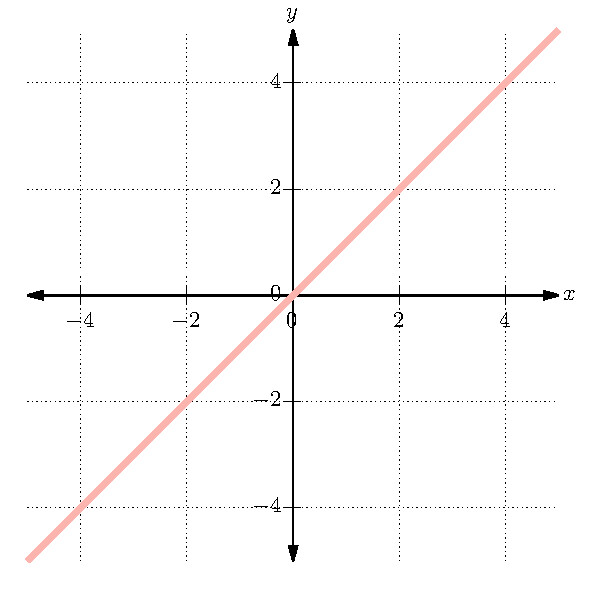
\includegraphics[scale=0.75]{function_graphs/f1.pdf}
  \end{figure}
  \item $f(x)=x^{2}$, not injective nor surjective.\\
  \textbf{Not injective}: For example, $f(3)=3^{2}=9=(3)^{2}=f(-3)$. In fact, each number $0\neq x\in\mathbb{R}$ has a non-unique image, since $x^{2}=(-x)^{2}$.\\
  \textbf{Not surjective}: Over $\mathbb{R}$, any negative number is not connected to by any input in the domain.
  \begin{figure}[H]
  \centering
  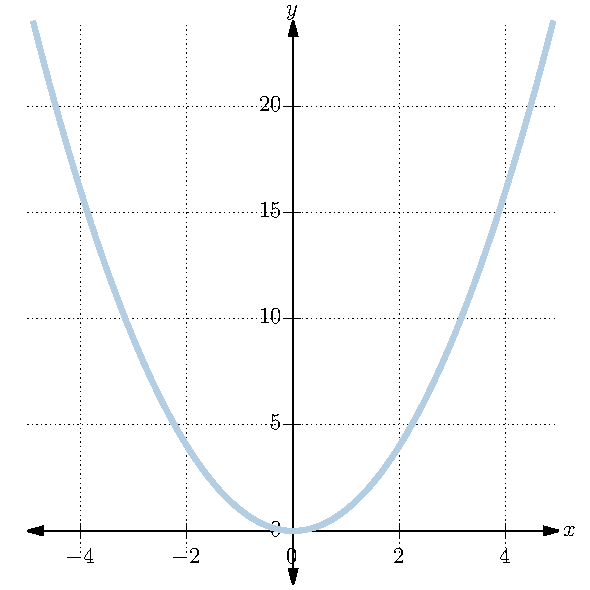
\includegraphics[scale=0.75]{function_graphs/f2.pdf}
  \end{figure}
  \item $f(x)=x^{3}$: injective and surjective $\Rightarrow$ bijective.
  \begin{figure}[H]
  \centering
  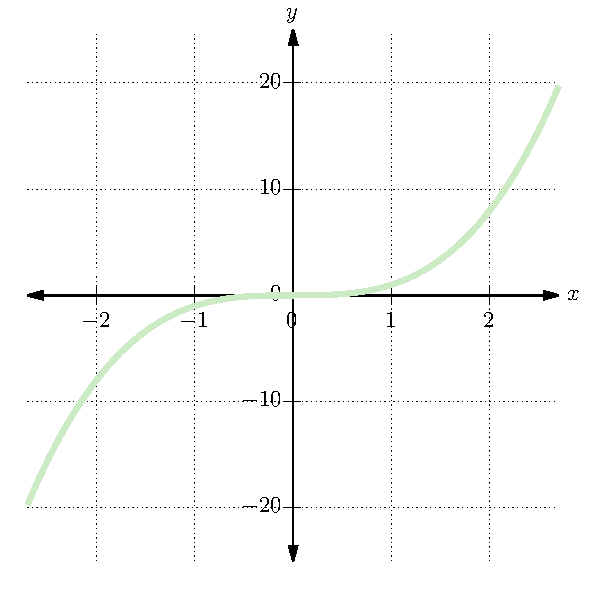
\includegraphics[scale=0.75]{function_graphs/f3.pdf}
  \end{figure}
  \item $f(x)=\cos(x)$, not injective nor subjective.\\
  \textbf{Not injective}: For example, $1=f(0)=f(2\pi)$.\\
  \textbf{Not surjective}: The actual image of $\cos(x)$ is $\left[ -1,1 \right]$, and over this interval it is surjective.
  \begin{figure}[H]
  \centering
  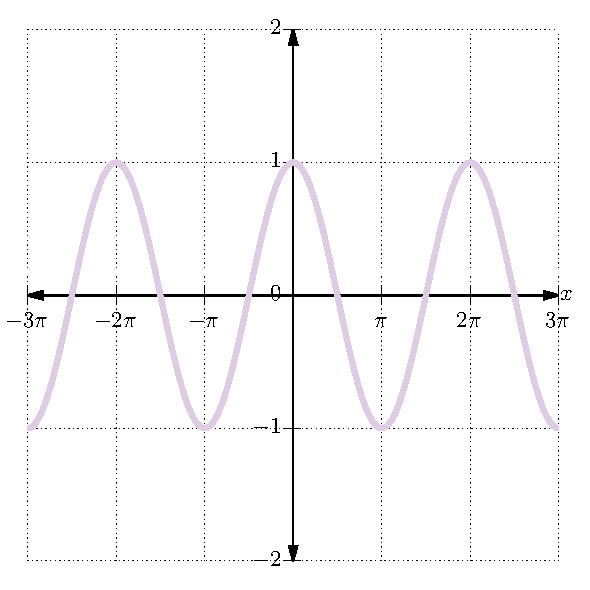
\includegraphics[scale=0.75]{function_graphs/f4.pdf}
  \end{figure}
  \end{itemize}
\end{example}

\subsection{Multivariable Functions}
Functions may have several arguments and return several arguments.
\begin{example}
  The follows functions take as input three real numbers, and return a single real number ($f:\mathbb{R}^{3}\to\mathbb{R}$). The return value of some functions for a triple of real numbers, $\left( -5,7,1 \right)$, are:
  \begin{itemize}
  \item $f\left( x,y,z \right)=x+y+z\Rightarrow f\left( -5,7,1 \right)=-5+7+1=3$
  \item $f\left( x,y,z \right)=x^{2}-y^{2}\Rightarrow f\left( -5,7,1 \right)=25-49=-24$
  \item $f\left( x,y,z \right)=\frac{x}{\sqrt{y}+z}\Rightarrow f\left(-5,7,1  \right)=\frac{5}{\sqrt{7}+1}$
  \end{itemize}
\end{example}
\begin{example}
  $f:\mathbb{Z}\times\mathbb{N}\to \mathbb{Q}$ is defined as follows: $f\left( p,q \right)=\frac{p}{q}$. The return value of $f$ for the some example inputs:
  \begin{itemize}
  \item $\left( 1,2 \right)\Rightarrow \frac{1}{2}=0.5$
  \item $\left( -5,2 \right)\Rightarrow \frac{-5}{2}=-2.5$
  \item $\left( 0,13 \right)\Rightarrow \frac{0}{13}=0$
  \end{itemize}
\end{example}

\section{Graphs}
\tikzset{
  between/.style args={#1 and #2}{
   at = ($(#1)!0.5!(#2)$)
  }
}
\def\dis{2.0cm}
\def\dText{0.3}

\emph{Graphs}\index{Graphs} are mathematical structures composed of \emph{nodes}\index{Nodes} (or \emph{vertices}\index{Vertex, vertices}, singular \emph{vertex}) connected to eachother by \emph{edges}\index{Edges}.
\begin{example}
  A graph with 5 nodes and 7 edges:
  \begin{figure}[H]
  \centering
  \begin{tikzpicture}[-, >=stealth', auto, node distance=\dis, semithick]
  \tikzstyle{every state}=[fill=col1, draw=black, very thick, text=black]
  \tikzstyle{every edge}=[draw=black, very thick]

  \node[state] (A)	  {A};
  \node[state] (B) [right=of A] {B};
  \node[state] (C) [below=of A] {C};
  \node[state] (D) [below=of B] {D};
  \node[state] (E) [between=B and D, xshift=2cm] {E};

  \path (A) edge node {} (B)
  (B) edge node {} (D)
  (C) edge node {} (A)
  (D) edge node {} (C)
  (E) edge node {} (B)
  (E) edge node {} (D)
  (A) edge node {} (D);

  \node[col1, left=of A] (nodetxt) {\textbf{Node (vertex)}};
  \node[above left=of C] (edgetxt) {\textbf{Edge}};
  \node[between=A and C] (edge) {};

  \draw[->, densely dotted, col1, thick] (nodetxt.east) to ($(A.west)+(-1mm,0)$);
  \draw[->, densely dotted, thick] (edgetxt.east) to (edge);
  \end{tikzpicture}
  \end{figure}
\end{example}

In the graphical representation of a graph, the actual position of nodes does not matter - what matters are the connections (edges) between them.

\begin{example}
  The follows are different representations of \textbf{the same} graph (3 nodes and 3 edges):
  \begin{figure}[H]
  \centering
  \begin{tikzpicture}[-, >=stealth', auto, node distance=\dis, semithick]
  \tikzstyle{every state}=[fill=col2, draw=black, very thick, text=black]
  \tikzstyle{every edge}=[draw=black, very thick]

  % First representation
  \node[state] (A1)	   {A};
  \node[state] (B1) [right=of A1]  {B};
  \node (AB1) [between=A1 and B1]  {};
  \node[state] (C1) [below=of AB1] {C};

  \path (A1) edge node {} (B1)
  (B1) edge node {} (C1)
  (C1) edge node {} (A1);
  
  % Second representation
  \node[state] (A2) [right=6cm of A1] {A};
  \node[state] (B2) [below=of A2] {B};
  \node[state] (C2) [below left=of B2]{C};

  \path (A2) edge node {} (B2)
  (B2) edge node {} (C2)
  (C2) edge node {} (A2);
  
  % Third representation
  \node[state] (A3) [right=3cm of A2] {A};
  \node[state] (B3) [below=of A3] {B};
  \node[state] (C3) [below=of B3] {C};

  \path (A3) edge node {} (B3)
  (B3) edge node {} (C3)
  (C3) edge [bend left]node {} (A3);
  \end{tikzpicture}
  \end{figure}
\end{example}

A graph where all edges have some direction is called a \emph{directed graph}\index{Directed graph}.
\begin{example}
  A directed graph with 4 nodes and 6 edges:
  \begin{figure}[H]
  \centering
  \begin{tikzpicture}[->, >=stealth', auto, node distance=\dis, semithick]
  \tikzstyle{every state}=[fill=col3, draw=black, very thick, text=black]
  \tikzstyle{every edge}=[draw=black, very thick]

  \node[state] (A) {A};
  \node[state] (C) [below=of A] {C};
  \node (AC) [between=A and C] {};
  \node[state] (B) [left=of AC] {B};
  \node[state] (D) [right=of AC] {D};

  \path (A) edge [bend left] node {} (B);
  \path (B) edge [bend left] node {} (A);
  \path (B) edge node {} (C);
  \path (C) edge node {} (D);
  \path (D) edge node {} (A);
  \path (D) edge [loop right] node {} (D);
  \end{tikzpicture}
  \end{figure}
\end{example}

\begin{warning}
  In a directed graph, an edge can "loop" back to a node. See node D in the example above.
\end{warning}

A \emph{path}\index{Path (graph theory)} in a graph is a sequence of edges in which each edge shares a vertex with the previous edge (except the first edge).
\begin{example}
  In the following graph the edges highlighted in red form a path:
  \begin{figure}[H]
  \centering
  \begin{tikzpicture}[auto, node distance=\dis, semithick]
  \tikzstyle{every state}=[fill=col4!50, draw=black, very thick, text=black]
  \tikzstyle{every edge}=[draw=black, very thick]

  \node[state] (1) {1};
  \node[state, below=of 1] (2) {2};
  \node[state, right=of 2] (3) {3};
  \node[state, above=of 3] (4) {4};
  \node[state, right=of 4] (5) {5};
  \node[state, below=of 5] (6) {6};
  \node[state, right=of 6] (7) {7};
  \node[state, above=of 7] (8) {8};
  
  \path (1) edge [ultra thick, red] node {} (2);
  \path (1) edge node {} (3);
  \path (1) edge node {} (4);
  \path (2) edge [ultra thick, red] node {} (3);
  \path (3) edge node {} (4);
  \path (3) edge [ultra thick, red] node {} (5);
  \path (3) edge node {} (6);
  \path (4) edge node {} (5);
  \path (5) edge [ultra thick, red] node {} (6);
  \path (5) edge node {} (8);
  \path (5) edge node {} (7);
  \path (6) edge [ultra thick, red] node {} (7);
  \path (7) edge [ultra thick, red] node {} (8);
  \end{tikzpicture}
  \end{figure}
\end{example}

When the start and end vertices coincide the path is known as a \emph{circle}\index{Circle (graph theory)}. A directed circle is known as a \emph{cycle}\index{Cycle (graph theory)}.

If one or more pathes exist between two vertices $a,b$ in a graph, the number of edges in the shortest path is defined to be the \emph{distance}\index{Distance (graph theory)} between the two vertices, and is denoted as $\dist(a,b)$.
\begin{example}
  In the following graph three paths between vertices 1 and 2 are shown. The number of edges in the shortest path, highlighted in red, is defined as the distance $\dist(1,2)$, and is equal to 3.
  \begin{figure}[H]
  \centering
  \begin{tikzpicture}[auto, node distance=\dis, semithick]
  \tikzstyle{every state}=[fill=col5!30, draw=black, very thick, text=black]
  \tikzstyle{every edge}=[draw=black, very thick]

  \node[state] (1) {1};
  \node[state, right=of 1] (a) { };
  \node[state, right=of a] (b) { };
  \node[state, right=of b] (2) {2};
  
  \path (1) edge [ultra thick, red] (a);
  \path (a) edge [ultra thick, red] (b);
  \path (b) edge [ultra thick, red] (2);
  
  \node[state, above right=of 1, xshift=-5mm] (c) { };
  \node[state, right=of c] (d) { };
  \node[state, right=of d] (e) { };
  
  \path (1) edge [ultra thick, col2!50!black] (c);
  \path (c) edge [ultra thick, col2!50!black] (d);
  \path (d) edge [ultra thick, col2!50!black] (e);
  \path (e) edge [ultra thick, col2!50!black] (2);
  
  \node[state, below right=of 1, xshift=-5mm] (f) { };
  \node[state, right=of f] (g) { };
  \node[state, right=of g] (h) { };
  
  \path (1) edge [ultra thick, col2!50!black] (f);
  \path (f) edge [ultra thick, col2!50!black] (g);
  \path (g) edge [ultra thick, col2!50!black] (h);
  \path (h) edge [ultra thick, col2!50!black] (2);
  \end{tikzpicture}
  \end{figure}
\end{example}

A \emph{tree}\index{Tree (graph theory)} is a graph with no circles.
\begin{example}
  A tree (notice that no circles are present):
  \begin{figure}[H]
  \centering
  \begin{tikzpicture}[auto, node distance=0.5*\dis, semithick]
  \tikzstyle{every state}=[fill=col3!30, draw=black, very thick, text=black]
  \tikzstyle{every edge}=[draw=black, very thick]

  \node[state] (1) { };
  \node[state, above left=of 1] (2) { };
  \node[state, above right=of 1] (3) { };
  \node[state, below=of 1] (4) { };
  \node[state, below left=of 4] (5) { };
  \node[state, below right=of 4] (6) { };
  \node[state, below=of 4] (7) { };
  \node[state, left=of 2] (8) { };
  \node[state, above right=of 3] (9) { };
  \node[state, below right=of 3] (10) { };

  \path (1) edge [ultra thick] (2);
  \path (1) edge [ultra thick] (3);
  \path (1) edge [ultra thick] (4);
  \path (4) edge [ultra thick] (5);
  \path (4) edge [ultra thick] (6);
  \path (4) edge [ultra thick] (7);
  \path (2) edge [ultra thick] (8);
  \path (3) edge [ultra thick] (9);
  \path (3) edge [ultra thick] (10);
  \end{tikzpicture}
  \end{figure}
\end{example}

Some trees have a distinctive \emph{root}\index{Root (graph theory)} node, and are known as \emph{rooted trees}\index{Rooted trees (graph theory)}. A node that is "branched" from a higher level node is called a \emph{child node}\index{Child node (graph theory)}. The last level nodes are called \emph{leaves}\index{Tree leaf} (singular: leaf). The rest of the nodes are known as \emph{inner nodes}\index{Inner nodes (graph theory)}.
\begin{example}
  A rooted tree, with the root node highlighted in red and the leaves in green:
  \tikzset{
  treenode/.style = {align=center, inner sep=0pt, text centered,
  font=\sffamily},
  tnode/.style = {treenode, circle, font=\sffamily\bfseries, draw=black,
  fill=col2!50, text width=1.5em},
  rnode/.style = {treenode, circle, font=\sffamily\bfseries, draw=black,
  fill=col1!50, text width=1.5em},
  lnode/.style = {treenode, circle, font=\sffamily\bfseries, draw=black,
  fill=col3!50, text width=1.5em},
  }
  \begin{figure}[H]
  \centering
  \begin{tikzpicture}[-, very thick, level/.style={sibling distance=2.5*\dis/#1, level distance=1.5cm}]
  \node [rnode] (root) { }
  child{ node (child1) [tnode] { }
  child{ node [tnode](child3) { }
  child{ node [lnode] { } edge from parent node[above left] {}}
  }
  child{ node [tnode] { }
  child{ node [lnode] { }}
  child{ node [lnode] {}}
  }
  }
  child{ node [tnode](child2)  { }
  child{ node [tnode] { }
  child{ node [lnode] { }}
  }
  child{ node [tnode] { }
  child{ node [lnode] { }}
  child{ node [lnode] {}}
  child{ node [lnode] (child4){}}
  }
  }
  ;

  \node[right=of root] (roottxt) {Root node};
  \draw[->,>=stealth, densely dotted, thick] (roottxt) to ($(root.east) + (2mm,0mm)$);
  
  \node[below=of root] (childtext) {Children of root};
  \draw[->,>=stealth, densely dotted, thick] (childtext) to ($(child1.east) + (2mm,0)$);
  \draw[->,>=stealth, densely dotted, thick] (childtext) to ($(child2.west) + (-2mm,0)$);

  \node[right=of child1.north] (br1) {};
  \node[right=of child3.south] (br2) {};
  \coordinate (A) at (-4.2,0);
  \draw[decorate, decoration={brace, amplitude=3pt, raise=9pt, mirror}]
  (A |- br1) -- (A |- br2) node[midway, xshift=-27pt, rotate=90] {Inner nodes};

  \node[right=of child4] (leaftxt) {Leaf node};
  \draw[->,>=stealth, densely dotted, thick] (leaftxt) to ($(child4.east)+(2mm,0)$);
  \end{tikzpicture}
  \end{figure}
\end{example}

Trees with 2 children per node are known as \emph{binary trees}\index{Binary trees}. Similarily, trees can be ternary, quaternary, etc.
\begin{example}
  A binary tree:
  \tikzset{
  treenode/.style = {align=center, inner sep=0pt, text centered,
  font=\sffamily},
  tnode/.style = {treenode, circle, font=\sffamily\bfseries, draw=black,
  fill=col2!50, text width=1.5em},
  }
  \begin{figure}[H]
  \centering
  \begin{tikzpicture}[-, very thick, level/.style={sibling distance=2.5*\dis/#1, level distance=1.5cm}]
  \node [tnode] (root) { }
  child{ node  [tnode] { }
  child{ node [tnode] { }
  child{ node [tnode] { }}
  child{ node [tnode] { }}
  }
  child{ node [tnode] { }
  child{ node [tnode] { }}
  child{ node [tnode] {}}
  }
  }
  child{ node [tnode]  { }
  child{ node [tnode] { }
  child{ node [tnode] { }}
  child{ node [tnode] { }}
  }
  child{ node [tnode] { }
  child{ node [tnode] { }}
  child{ node [tnode] {}}
  }
  }
  ;
  \end{tikzpicture}
  \end{figure}
\end{example}

Rooted trees are used to describe hierarchies, e.g. in biological systematics, organisations or nested directories of data.

The \emph{complete graph}\index{Complete graph} $K_{n}$ is the graph with $n$ vertices where every pair of different vertices is connected by an edge (Also called a \emph{clique}\index{Clique (graph theory)}).

\begin{example}
  The cliques $K_{1}, \dots, K_{6}$:
  \newcommand{\clique}[3]{
  \pgfmathsetmacro{\ang}{180-((#1-2)*180/#1)}
  \pgfmathsetmacro{\rad}{#2}
  \pgfmathsetmacro{\anull}{90}
  \pgfmathsetmacro{\xnull}{#3}

  \foreach \n in {1,...,#1}{
  \node[circle, font=\sffamily\bfseries, draw=black, very thick, fill=col2!50, text width=0.25em] (p\n) at ({#2*cos(\n*\ang+\anull)+\xnull},{#2*sin(\n*\ang+\anull)}) { };
  \foreach \m in {1,...,\n}{
  \draw[-, very thick] (p\n) to (p\m);
  }
  }
  
  \node at (\xnull,-1.5cm) {$K_{#1}$};
  }

  \begin{figure}[H]
  \centering
  \begin{tikzpicture}
  \foreach \K in {1,...,6}{
  \clique{\K}{0.75}{\K*2.5}
  }
  \end{tikzpicture}
  \end{figure}
\end{example}
